\chapter{Photoassociation spectroscopy: theory and methods}
\label{ch:chap3}

\section{Introduction}
\label{sec:pas_intro}

This part needs to be brief and really should motivate the idea of PAS.

Okk, first ogg we introduce the potential between atoms

this arises from the interaction of scattering theory with a molecular state. ''the interaction potential between two atoms. Ehich is caused by?

this results in a poitential that supports bound states . In atomic physics, our low density fases are mainly within the regime of small interactions. This spatial dependence is mapped onto the internal energy levels of each atom. I want to say dressed state model here (review atom-photon coupling, atomic physics book).

Definitely need some BS about how simple scattering theory has been a hallmark of atomic physics and 

What about the history of scattering? Most of what we know about quantum mechanics comes from either scattering experiments of spectroscopy. Photoassociation spectroscopy is an important field which relies on both of these properties.

\subsection{PAS in atomic physics}
\label{ssec:pas_amo}

PA is not unique to atomic physics, chemists have been using light to interrogate molecular structure for a long time

physicists molecule, short-range PA, rabi oscilations between atomic and molecular condensates (cite ours and the lattice experiment that followed)

Pioneering work done in the early 90's used PA to interrogate the sturucture of interatomic potentials to deduce the scattering lengths between atoms. 

Can even be used to modify the scattering length of atoms through mixing of atomic eigenstates.

This work is focused on long-range PA but in recent years groups have also developed short-range PA techniques for the creation of ro-vibrational ground state molecules. These techniques rely heavily on favorable overlap integrals betwwen molecular wavefunctions and typically searching for favorable intermediate states is a pain (that is why our large FCF might be useful)

There are multiple flavors of PAS. Can do one-photon or two-photon. 

\subsection{Low energy two-body scattering}
\label{ssec:scattering}

consider the two particle system as a single entagled particle
	long range part of this quasi-particle is just the eigenstates of the separate particles themselves (only composed of two parts)
	but the short range part is going to be determined by some complex physics (new eigenstates, what is the coupling mechanism?)
		the vdW point is the boundary distance?
		coupling is due to the interatomic potential, there is at least the long-range part falling off as R6, what are the types of interactions which make up the internal wall?


Think I want to introduce the photoassocation by talking about the collisional wavefunction

what will that do?

I want to build up ideas about the FCF and need the wf for that
	to get qf I have to go back to scattering theory

ideas of the wavefunction become that basis for how you want to talk about interacting potentials


free atoms
scatering as single particle state (differnet eigenstate)
	interaction determined by some gnarly stuff
From scattering theory we know that the long range behavior is determined by short range physics
	how do we know this? (the dalibard intro)
Can we come up with good enough pseudo potentials to describe the short range physics and then solve the schrodinger equation to extract wavefunctions?
	we want wavefunctions because that is the full characterization
	we don't know the right eigenbasis for the short range part but we can make some guesses (in particular Hund cases setup eigen states for various possible internal states)
	Bohn and Julienne theory guessed based on using quantum defect theory
		this pre-supposes that the bound and free wavefunctions are similar (I forget in what respect) but that the bound ones must go to zero as R->Inf
If we have some notion of the wf then we can construct matricies which define interactions once we add additional coupling to the scattering problem


now in a position where I need to connect scattering theory and the PAS


Once we have the ground state wavefunction of our new particle we can construct the internal structure by considering the internal energy strucutrue of the constituent atoms
	Can I make a connnection that since it is a composite particle we must consider all the various configurations available?
	
\begin{figure} \label{fig:ch3_sr_scat_wf}
	\centerline{
	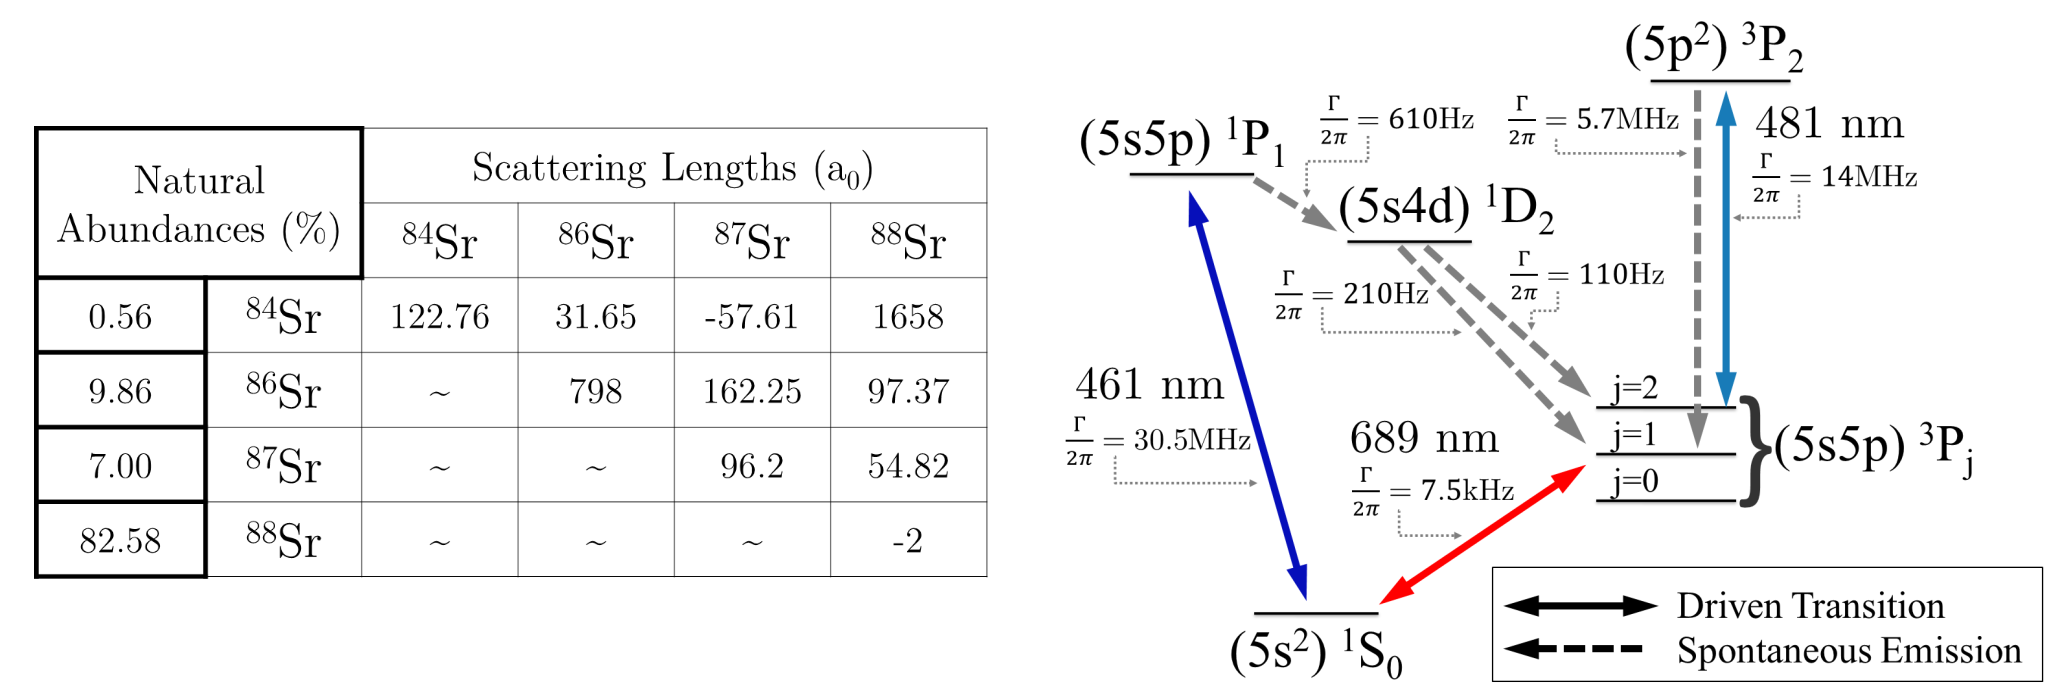
\includegraphics[height=0.25\textheight]{strontium_properties.pdf}}
	\caption{Strontium interatomic wavefunctions}{Res 6.3}
\end{figure} 

\subsection{Modifying interactions}
\label{ssec:mod_int}

Also the Chin '10 review on feshbach resonances

Follow the Nicholson 15 paper method of introing the elastic and inelastic cross sections

\section{Semi-classical treatment of lineshapes}
\label{sec:bohn_and_julienne}

Now that we have the theory of PAS covered. PA can come in many forms (in a lattice, in a bulk gas, via dissociating molecules) Experimentally we observe PA by looking for trap loss \hl{doublon paper}.

This section will cover the theory of lineshapes in PAS.

Somewhere I read about three regimes of PAS as a comparison of relevant energy scales. Should explore that here

\begin{equation}\label{number}
   N(t)={N_0 \rm{e}^{-\Gamma t} \over 1+
   {2 N_0 \langle K \rangle V_2\over \Gamma V_1^2}(1-\rm{e}^{-\Gamma t})}
\end{equation}
where  $N_0$  is the number  at the beginning of the PAS interaction
time, and $\langle K \rangle$ indicates a spatial average of collision event rate constant $K$ (Eq.\ \ref{equationKeffective}). The one-body loss rate, $\Gamma$, is due to background
collisions and off-resonant scattering from the PA lasers.

PA loss is described with a local equation for the evolution of the atomic density [Eq.~(\ref{densitydecay})]. Integrating Eq.~(\ref{densitydecay}) over the trap volume yields the time evolution of the number of trapped atoms [Eq.~(\ref{number})]. The effective volumes used throughout this analysis are defined by
\begin{equation}\label{eq:effectivevolumes}
	V_{\text{q}}=\int_{\mathrm{V}} d^3r \, e^{-\frac{qU(\mathbf{r})}{k_{B}T}},
\end{equation}
for trapping potential $U(\mathbf{r})$. The collision event rate constant can be expressed as a thermal average of the scattering probability for loss, $\vert S(\epsilon,\omega_1,\omega_2,...,\mathbf{r})\vert^2$, over the collision energy $\epsilon$. We also average over the trap volume to allow for the possibility that the scattering probability can vary with position in the trap due to inhomogeneity of laser intensity profiles and the density distribution [Eq.~(\ref{equationKeffective})].

%This yields
\begin{eqnarray}\label{equationKeffective}
% \nonumber to remove numbering (before each equation)
  \langle K \rangle&=& \frac{1}{V_{2}}\int_{\mathrm{V}}
d^3r \,
          e^{-\frac{2U(\vec{r})}{k_{B}T}} \nonumber \\
         &&\times \frac{1}{h\,Q_{T}}
\int_{0}^{U_{max}-U(r)}d\epsilon \vert S\vert^2
   \,e^{-\epsilon/k_{B}T}.
\end{eqnarray}
%\begin{equation}\label{Kintegral}
%   K=\frac{1}{h\,Q_{T}} \int \vert S(\epsilon,\omega_1,\omega_2,...)\vert^2
%   \,e^{-\epsilon/k_{B}T} \; d\epsilon,
%\end{equation}
where the partition function is $Q_{T}=\left({2\pi k_{B}T \mu \over
h^2}\right) ^{3/2}$ for reduced mass $\mu$.


Bohn and Julienne \cite{bju96} provide an expression for $\vert S(\epsilon,\omega_1,\omega_2,...)\vert^2$ for a collision on the open channel of two ground state atoms (g) with total energy $\epsilon$ leading to loss-producing decay from the excited state $b_1$ with rate $\gamma_1$. (See Fig.\ \ref{PASDiagram}.) It yields
\begin{eqnarray}\label{equationSprob}
  \vert S\vert^2 =   \hspace{2.5in}&&\\
  {(\Delta_2+\epsilon/\hbar)^2{\gamma}_1{\gamma}_s \over
  	\left[(\Delta_1+\epsilon/\hbar)(\Delta_2+\epsilon/\hbar)-\frac{\Omega_{12}^{2}}{4}\right]^2+\left[ \frac{\gamma_1+\gamma_s}{2}\right]^2(\Delta_2+		 	\epsilon/\hbar)^2}, &&\nonumber
\end{eqnarray}
where all quantities are defined in the main text. For simplicity, we have omitted the light shift of $b_1$ due to coupling to the scattering continuum \cite{bju99}. Equation (\ref{equationSprob}) neglects all light shifts due to the trapping laser. Light shifts due to the photoassociation lasers coupling to states outside our model (Fig.\ \ref{PASDiagram}) are also neglected. The thermal energy is much greater than the zero-point energy for trap motion, $T\gg h\nu_{\text{trap}}/k_B$, so confinement effects are negligible \cite{zbl06}.

%$\Delta_1=\omega_1-E_{b1}/\hbar$ and $\Delta_2=\omega_1-\omega_2-E_{b2}/\hbar$ are the one-photon detuning from state $b_1$ and two-photon detuning from state $b_2$ respectively for initial scattering state with $\epsilon=0$.

%, which is a good approximation for our experiment because the light shift of state 1 is small compared to the detuning $\hbar \Delta_1$,
and lights shifts of states 0 and 2 are approximately equal and will cancel in the determination of the binding energy of the halo state, $E_2$ \cite{rbm04,rfk87}. Neglecting

%We record spectra by varying $\Delta_2$ at fixed detuning from the intermediate state $\Delta_1$

For the experiments reported here, we maintain significant intermediate-state detuning, $|\Delta_1|\gg |\Omega_{12}|$. Thus we are in a Raman configuration, and near two-photon resonance the expression for the scattering probability for a given initial scattering energy Eq.~(\ref{equationSprob}) can be approximated as a Lorentzian
\begin{eqnarray}\label{equationSprobLorentzian}
 \vert S\vert^2 \approx {A(\epsilon) \over
 \left(\Delta_2+\epsilon/\hbar-\frac{\Omega_{12}^{2}}{4(\Delta_1+\epsilon/\hbar)}\right)^2+\left[ {\Gamma_L(\epsilon)}/{2}\right]^2},
\end{eqnarray}
where $A$ and $\Gamma_L$ are defined in Eqs.\ (\ref{ApproxLorentzianQuantitiesMain}) and (\ref{ApproxLorentzianQuantities-2Main}).

As discussed in the text, we analyze loss spectra using the effective expression, Eq.\ (\ref{equationApproxLorentzian}) to account for possible deviations from the single-channel theory \cite{bju96}.

%\section{AC Stark shift due to excitation lasers}
\label{App:ACStark}
The total 689-nm intensity oscillates with 100\% contrast according to
$I_{total}=I_1+I_2+2\sqrt{I_1I_2}\cos \left[(\omega_1-\omega_2)t \right]=2I\left\{1+\cos \left[(\omega_1-\omega_2)t \right]\right\}$.
Equation \ref{Eq:ACStarkFullModel}
The form of the AC Stark shift
due to excitation lasers in Eq.\ \ref{Eq:GlobalFit}
 reflects the time average of the intensity and neglects the interference term. To confirm that this is the correct description, we numerically solved the time-evolution for a three-level system with similar optical couplings and oscillating optical intensity as present during halo photoassociation. The Hamiltonian is
\begin{eqnarray}\label{Eq:ThreeLevelHamiltonian}
H= \hspace{3in} \\
 \nonumber\\
\left(
    \begin{array}{ccc}
      0 & \Omega_{01}\left[\mathrm{cos}(\omega_1 t)+ \mathrm{cos}(\omega_2 t)\right] & 0 \\
      . & E_{b1} & \Omega_{12}\left[\mathrm{cos}(\omega_1 t)+ \mathrm{cos}(\omega_2 t)\right] \\
      . & . & E_{b2} \\
    \end{array}
  \right)
\nonumber
\end{eqnarray}
For  $\Omega_{01}\ll \Omega_{12} \ll \Delta_{1}\equiv E_{b1}/\hbar-\omega_1$, which is analogous to the  experimental conditions used here

, the shift of the two-photon resonance condition follows $\delta={\Omega_{12}^{2}}/{2\Delta_{1}}$ in agreement with Eq. \ref{Eq:ACStarkFullModel}.

\section{Observing photoassociative loss}
\label{sec:pa_methods}

In this work, we probe the halo state in 86Sr using two-photon Raman photoassociation (PA) \hl{cite 16 from halo paper}, in which two laser fields couple colliding atoms to the least-bound state of the ground molecular potential. We tune near resonance with an intermediate state that is bound in the 0u potential corresponding to the \intPot{\gs}{\ex} asymptote at long range as shown in Fig.\ref{fig:ch3_sr_pas}.

\begin{figure} \label{fig:ch3_sr_pas}
	\centerline{
	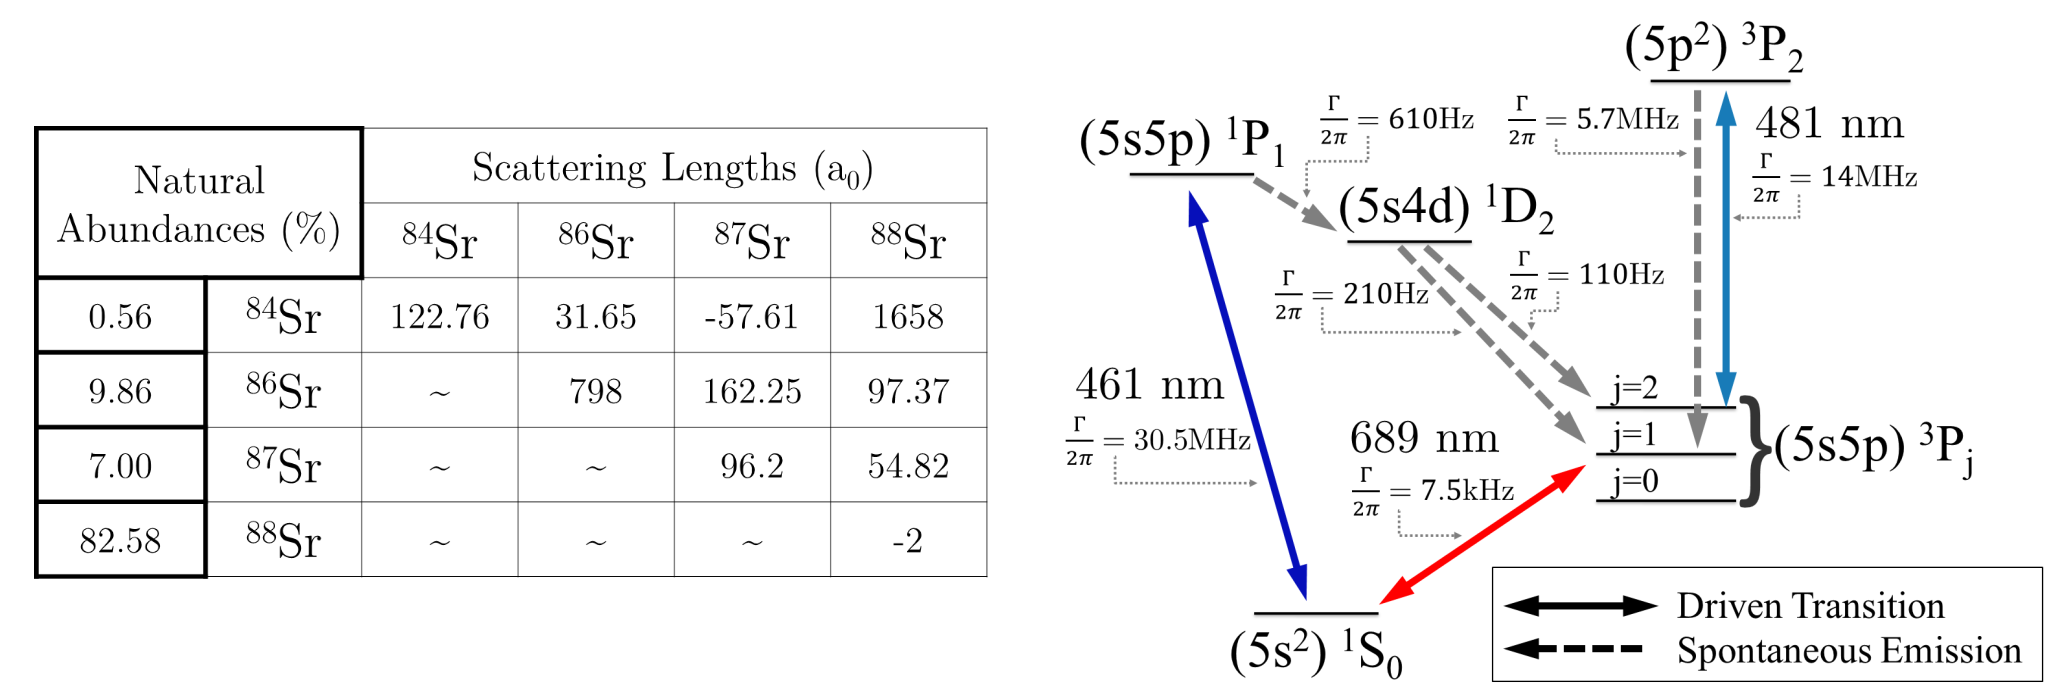
\includegraphics[height=0.25\textheight]{strontium_properties.pdf}}
	\caption{Strontium two-photon photoassociation}{fig 1 from the halo paper}
\end{figure} 

Photoassociation experiments follow the same general presciprtion. We start by trapping through the normal sequence as outlined in \hl{some section}. Then we evaporate down to the final trap depth. After evaporation 

The two-photon PAS experiments described in the following chapters are performed under similar conditions but due to complications with the neutral vaccuum system we performed the binding energy experiemtns using the Rydberg apparatus. While non-ideal from a consistency point of view, this did allow us to replicate and validate our previous findings which gives us great confidence in the robustness of this experimental appraoch. 

The most significant difference between the two apparatus' is the trapping characteristics of the optical dipole traps and the beam parameters of the photoassociation beam. These differences are noted in the corresponding chapters but here we will outline the timing and generic characteristics that are shared between the two experiments. 

Table \hl{something} shows the relevant experimental parameters and typical values for our photoassociation experiments. 

Specific details of the optical dipole traps, PA beam parameters, and using a completely different a 

 performed on ultracold Sr atoms in a single-beam optical dipole trap (ODT) generated from a 1064-nm laser propagating perpendicular to gravity. Typical atom numbers are several hundred thousand and peak densities are $\approx \peakDens{1}{12}$. The number of atoms and sample temperature are measured using time-of-flight absorption imaging described in \hl{some section}. Trap oscillation frequencies are determined by measuring dipole and breathing collective mode frequencies, which allow determination of trap volume and sample density



For experiments done on our apparatus we generate the two photon source as shown in Fig\ref{fig:pas_light_gen}. Light comes from an injection locked slave diode which follows the frequency stablized 689 master laser described in \hl{some section}. THis light is modulated via a single acousto-optic modulator (AOM) driven with two frequencies and coupled into a single-mode polarization maintaining optical fiber. THis fiber output is luanched near the science chamber and the light output level is continuously monitored via a beam sampler and photodiode placed between the fiber output and the chamber.

\begin{figure} \label{fig:ch3_pas_light_gen}
	\centerline{
	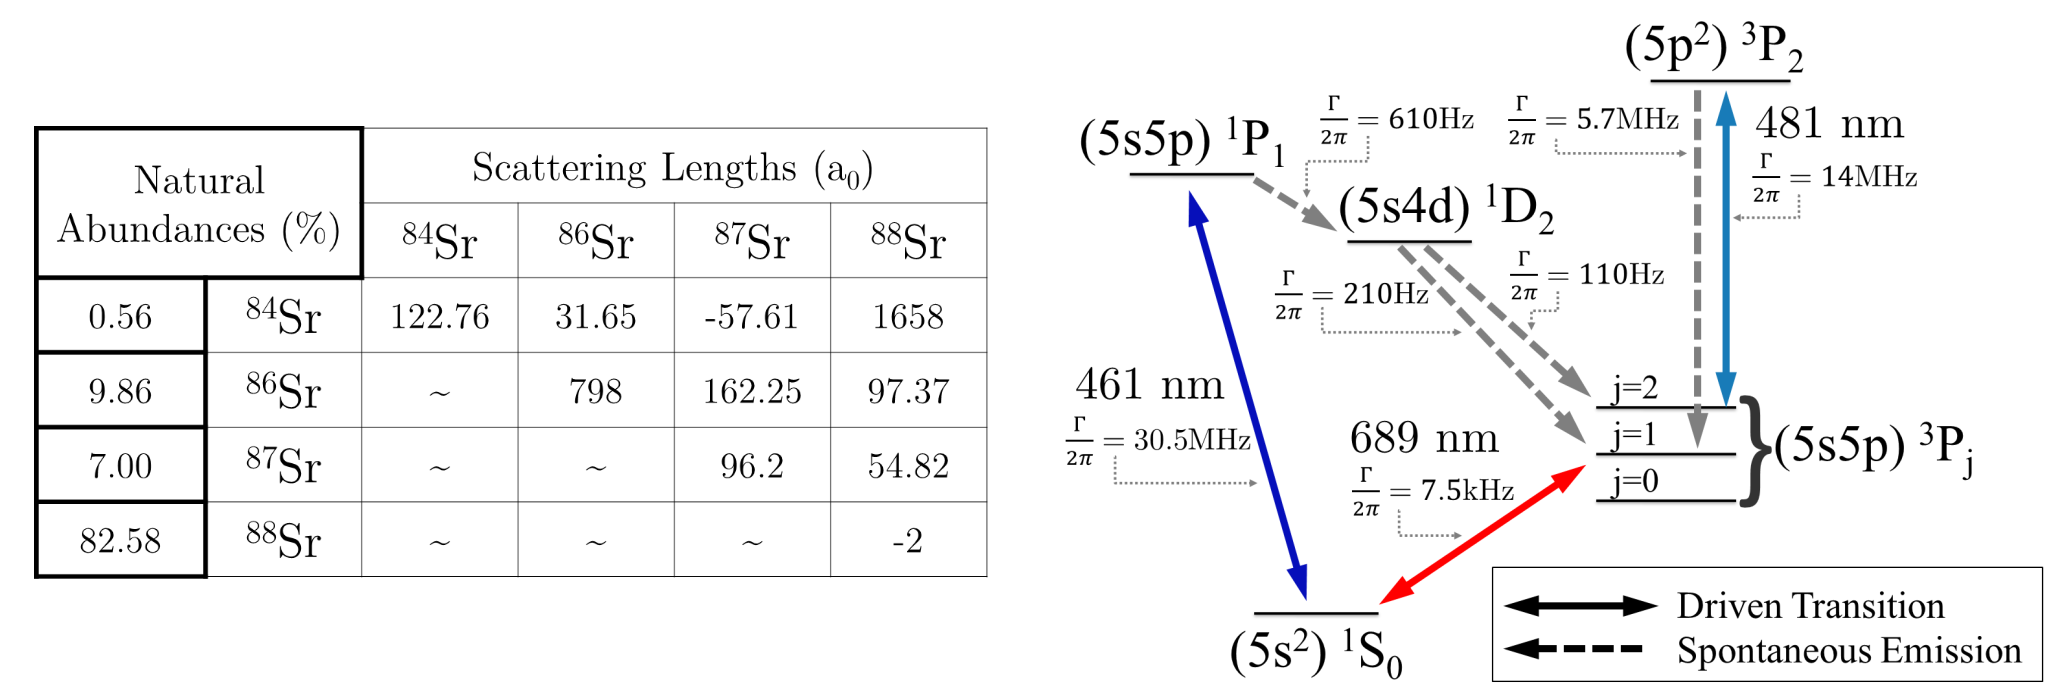
\includegraphics[height=0.25\textheight]{strontium_properties.pdf}}
	\caption{Schematic of PAS light generation}{Properties of strontium. Left: Natural abundances and s-wave scattering lengths for all mixtures of Sr. Right: Simplified energy level diagram of Sr showing the relevant states used for trapping and cooling of the atomic gas}
\end{figure} 

Primary reasons why we can't scan large distances. There will be a slight misalignment of the beams into the fiber and the RF may start to fall off. For these experiments an AOM with a center frequecny of 90 MHz was used. 

This simple system has many advantages and a couple of drawbacks. Since both photons are aligned into the same fiber then they are gauranteed to have the same output wavevector and therefore the two photon process will be doppler free (since the absorption and emission processes will exactly cancel each other out).

This is a simple system for generating multiple frequencies which are gauranteed to share the same wavevector, phase coherence, and gross frequency stability. Use of the AOM provides highly accurate control of the difference frequency with RF precision. 

While versatile and simple, we are worried about the balnace of the RF power onto the AOM. THese devices are narrowband modulators (simple ones) 

We see a reduction in contrast when the two drive frequencies differ by more than $\approx$250 kHz. 

Since the modulator is a narrowband device, scann

great care is taken to ensure the maximum amount of contrast is visible on the photodiode. This 

As described in \hl{some section} the slave laser is frequency stabiliezed at +42 MHz of the 86Sr $\gs\,\rightarrow\,\ex$ atomic transition. The AOM then shifts the light the remaining $\approx$ 86 MHz to set the detuning around the $\nu=-2$ bound state of the \intPot{\gs}{\ex} potential. Setting of $\Delta_1$ is done by removing one of the frequencies, peaking up the diffraction angle and alignment into the fiber. 

During the course of our experiments we found that mild environmental perturbations (loud noises, air currents due to fans, etc.) to the fiber resulted in slow variation of the light coupling through the fiber. Such amplitude modulations are not uncommon in laser systems and can typically be  compensated for by using a closed loop locking mechanism. However, after construction of such a power lock the compoenets did not react quickly enough and there was a significant overshoot which resulted in an uncontrolled amount of light illuminating the atoms during short exposures. This led us to implement a digital based sample and hold mechanism for reduced intensity variability. This system is described in detail in \hl{some section}. The sample and hold system in combination with the power lock provided intensity stability with a standard 5\% standard deviation during a typical experiment. Fig shows a typical histogram of the recorded intensities. 

Make sure to discuss how I scanned the rf frequencies since there is a difference to increasing the freq difference. Since we used the -1 order of the AOM, increasing the frequency of the drive relative to the gross actually lowered the amount of energy in the system, resulting in effectively scanning $\Delta_1$ instead of keeping it fixed. This resulted in a slight variation of the AC stark shift from the intermediate state that can be seen in the strong coupling experiments that are discussed in \hl{some section}. 

\begin{figure} \label{fig:ch3_pas_histogram}
	\centerline{
	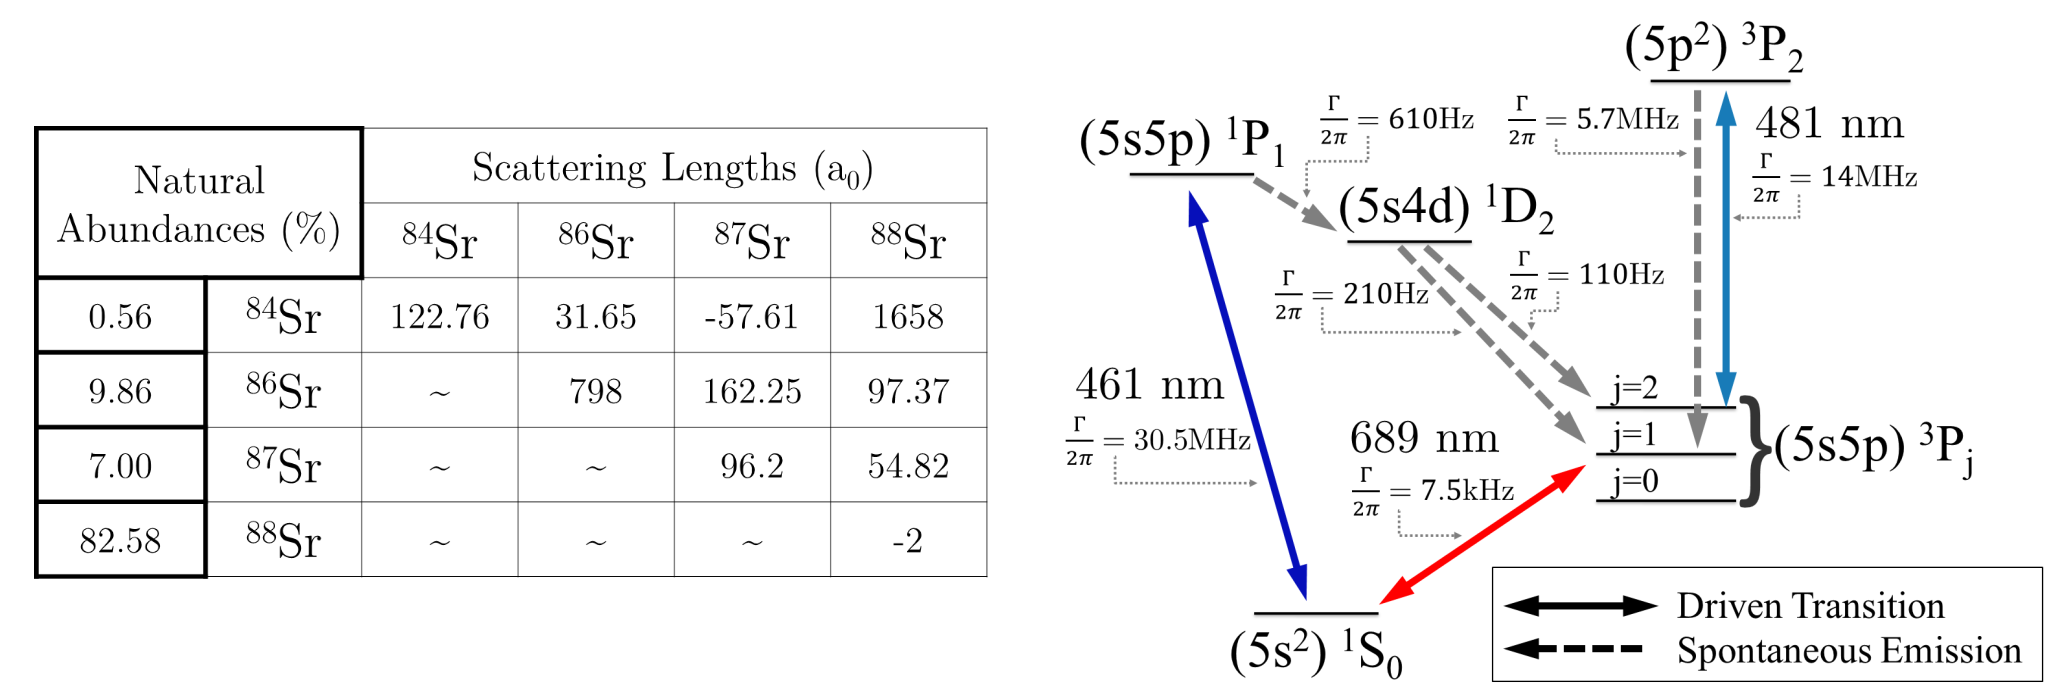
\includegraphics[height=0.25\textheight]{strontium_properties.pdf}}
	\caption{Histogram of PAS beam intensity variation}{One of the histograms from onenote. There are separate histograms for each experimental run (I should combine this so I don't have to disucss)}
\end{figure} 

The beat signal of the two light fields after the fiber is monitored on a photodiode and the rf powers are adjusted to ensure matched intensities for the two frequency components ($I_1 = I_2 \equiv I$).

\begin{figure} \label{fig:ch3_pas_light_balance}
	\centerline{
	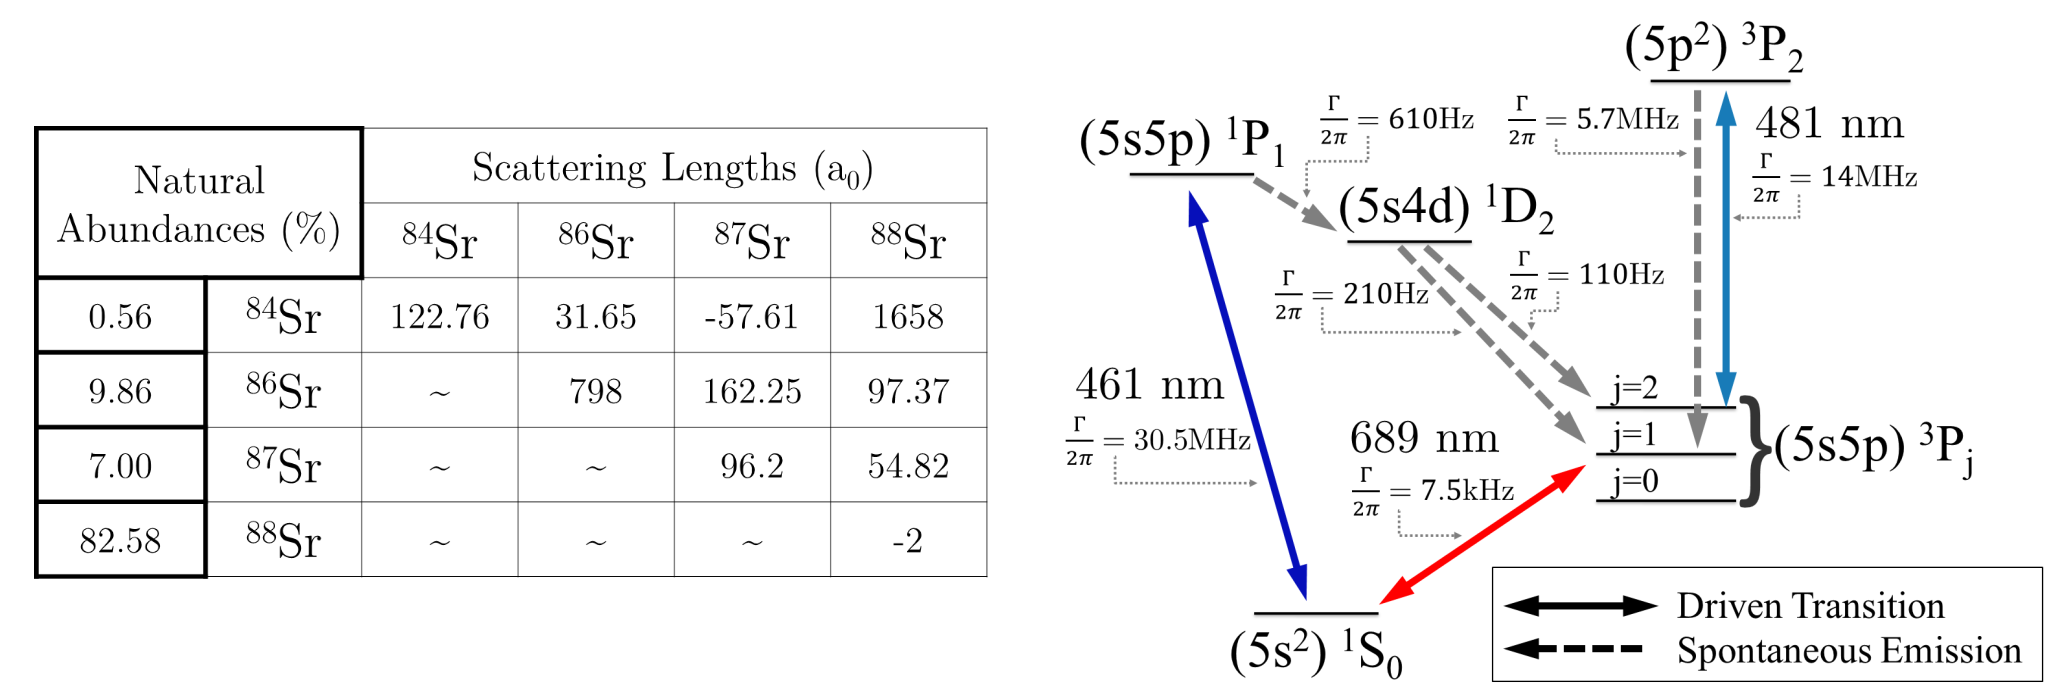
\includegraphics[height=0.25\textheight]{strontium_properties.pdf}}
	\caption{Characteristic view of the PA beatnote}{This is the picoscope plot of the beatnote}
\end{figure} 

